%codigo fixo
\documentclass{beamer}
\usepackage{tikz}
\usepackage{xcolor}
\usetheme{default}
\beamertemplatenavigationsymbolsempty

%definição das cores dos planetas
\definecolor{sol} {rgb}{0.992156863,0.792156863,0.003921569}
\definecolor{mercurio} {rgb}{0.850980392,0.733333333,0.478431373}
\definecolor{venus} {rgb}{0.992156863,0.792156863,0.003921569}
\definecolor{terra} {rgb}{0.003921569,0.2,0.592156863}
\definecolor{marte} {rgb}{1,0.207843137,0.003921569}
\definecolor{jupiter} {rgb}{0.505882353,0.4,0.278431373}
\definecolor{saturno} {rgb}{0.850980392,0.733333333,0.478431373}
\definecolor{urano} {rgb}{0.4,0.4,0.4}
\definecolor{netuno} {rgb}{0.003921569,0.411764706,0.788235294}


%distancia do sol
%mercurio   1.5
%venus      2
%terra      2.5
%marte      3
%jupiter    3.7
%saturno    4.7
%urano      5.5
%netuno     6


\begin{document}
      \begin{frame}
            \transduration{0.71}
            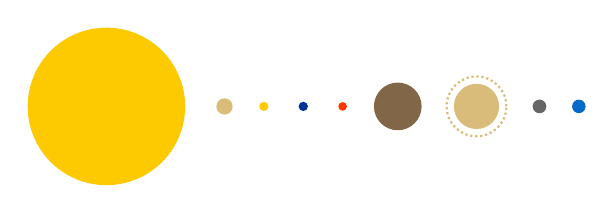
\begin{tikzpicture}
                  \fill[sol] (1,7) circle(10.00000000mm);
                  \fill[mercurio] (2.5,7) circle(1.035053161mm);
                  \fill[venus] (3,7) circle(0.586951149mm);
                  \fill[terra] (3.5,7) circle(0.591639368mm);
                  \fill[marte] (4,7)      circle(0.548795977mm);
                  \fill[jupiter] (4.7,7) circle(3.027183908mm);
                  \draw[saturno,thick,densely dotted] (5.7,7) circle(3.797758621mm);
                  \fill[saturno] (5.7,7) circle(2.86591954mm);
                  \fill[urano] (6.5,7) circle(0.867227011mm);
                  \fill[netuno] (7,7) circle(0.855804598mm);
            \end{tikzpicture}
      \end{frame}
\end{document}